\section{APIs}
\label{api}

Im folgenden wird häufig die Rede sein von APIs.
Daher soll hier kurz geklärt werden, was eine API ist und wie diese im Allgemeinen funktionieren.
API steht kurz für Application Programming Interface (Programmierschnittstelle)~\cite[vgl.]{api}.
Eine API ermöglicht es, dass unabhängige Anwendungen miteinander kommunizieren und Daten austauschen können~\cite{api}.
Im allgemeinen funktioniert diese Kommunikation mit dem HTTP-Protokoll über das Internet.
Dabei stellt ein System per HTTP eine Anfrage und die API liefert eine Antwort.
Es ist nicht festgelegt, auf welche Art das System die Antwort für die API erzeugt.
Dies hängt stark von der zugrundeliegenden Implementierung ab.

\begin{figure}[h!]
    \centering
    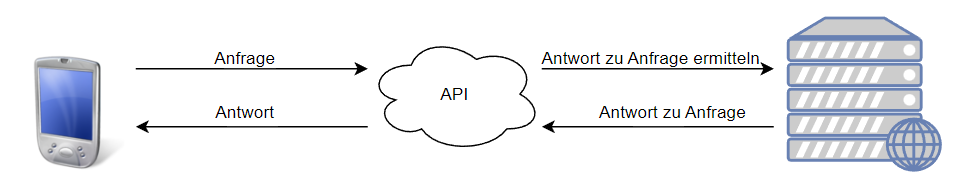
\includegraphics[width=\textwidth,height=\textheight,keepaspectratio]{img/webapi}
    \caption{simple API-Kommunikation}
    \label{basicapi}
\end{figure}

Es gibt verschiedene Entwurfsmuster, die man für ein API Design nutzen kann.
Die verschiedenen Muster werden durch Programmcode umgesetzt und sind somit fehleranfällig.
In dieser Arbeit wird die Umsetzung von GraphQL-APIs betrachtet und der Programmcode hinter der GraphQL-API
soll automatisiert getestet werden, sodass die Softwarequalität von der Programmierschnittstelle verifiziert werden kann.

\newpage